\documentclass[12pt]{article}

%%%%%%%%%%%%%%%%%%%%%%%%%%%%%%%%%%%%%%%%%%%%%%%%%%%%%%%%%%%%%%%%%%%%%%%%%%%%%%%%
%                           Package preset for homework
%%%%%%%%%%%%%%%%%%%%%%%%%%%%%%%%%%%%%%%%%%%%%%%%%%%%%%%%%%%%%%%%%%%%%%%%%%%%%%%%
% Miscellaneous
\usepackage[margin=1in]{geometry}
\usepackage[utf8]{inputenc}
\usepackage{indentfirst}
\usepackage{blindtext}
\usepackage{graphicx}
\usepackage{xr-hyper}
\usepackage{hyperref}
\usepackage{enumitem}
\usepackage{color}
\usepackage{float}
% Math
\usepackage{latexsym}
\usepackage{amsfonts}
\usepackage{amssymb}
\usepackage{amsmath}
\usepackage{commath}
\usepackage{amsthm}
\usepackage{bbold}
\usepackage{bm}
% Physics
\usepackage{physics}
\usepackage{siunitx}
% Code typesetting
\usepackage{listings}
% Citation
\usepackage[authoryear]{natbib}
\usepackage{appendix}
\usepackage[capitalize]{cleveref}
% Title & name
\title{Homework}
\author{Tien Vo}
\date{\today}


%%%%%%%%%%%%%%%%%%%%%%%%%%%%%%%%%%%%%%%%%%%%%%%%%%%%%%%%%%%%%%%%%%%%%%%%%%%%%%%%
%                   User-defined commands and environments
%%%%%%%%%%%%%%%%%%%%%%%%%%%%%%%%%%%%%%%%%%%%%%%%%%%%%%%%%%%%%%%%%%%%%%%%%%%%%%%%
%%% Misc
\sisetup{load-configurations=abbreviations}
\newcommand{\due}[1]{\date{Due: #1}}
\newcommand{\hint}{\textit{Hint}}
\let\oldt\t
\renewcommand{\t}[1]{\text{#1}}

%%% Bold sets & abbrv
\newcommand{\N}{\mathbb{N}}
\newcommand{\Z}{\mathbb{Z}}
\newcommand{\R}{\mathbb{R}}
\newcommand{\Q}{\mathbb{Q}}
\let\oldP\P
\renewcommand{\P}{\mathbb{P}}
\newcommand{\LL}{\mathcal{L}}
\newcommand{\FF}{\mathcal{F}}
\newcommand{\HH}{\mathcal{H}}
\newcommand{\NN}{\mathcal{N}}
\newcommand{\ZZ}{\mathcal{Z}}
\newcommand{\RN}[1]{\textup{\uppercase\expandafter{\romannumeral#1}}}
\newcommand{\ua}{\uparrow}
\newcommand{\da}{\downarrow}

%%% Unit vectors
\newcommand{\xhat}{\vb{\hat{x}}}
\newcommand{\yhat}{\vb{\hat{y}}}
\newcommand{\zhat}{\vb{\hat{z}}}
\newcommand{\nhat}{\vb{\hat{n}}}
\newcommand{\rhat}{\vb{\hat{r}}}
\newcommand{\phihat}{\bm{\hat{\phi}}}
\newcommand{\thetahat}{\bm{\hat{\theta}}}

%%% Other math stuff
\providecommand{\units}[1]{\,\ensuremath{\mathrm{#1}}\xspace}
% Set new style for problem
\newtheoremstyle{problemstyle}  % <name>
        {10pt}                   % <space above>
        {10pt}                   % <space below>
        {\normalfont}           % <body font>
        {}                      % <indent amount}
        {\bfseries\itshape}     % <theorem head font>
        {\normalfont\bfseries:} % <punctuation after theorem head>
        {.5em}                  % <space after theorem head>
        {}                      % <theorem head spec (can be left empty, 
                                % meaning `normal')>

% Set problem environment
\theoremstyle{problemstyle}
\newtheorem{problemenv}{Problem}[section]
\newenvironment{problem}[1]{%
  \renewcommand\theproblemenv{#1}%
  \problemenv
}{\endproblemenv}
% Set lemma environment
\newenvironment{lemma}[2][Lemma]{\begin{trivlist}
\item[\hskip \labelsep {\bfseries #1}\hskip \labelsep {\bfseries #2.}]}{\end{trivlist}}
% Set solution environment
\newenvironment{solution}{
    \begin{proof}[Solution]$ $\par\nobreak\ignorespaces
}{\end{proof}}
\numberwithin{equation}{problemenv}

%%% Page format
\setlength{\parindent}{0.5cm}
\setlength{\oddsidemargin}{0in}
\setlength{\textwidth}{6.5in}
\setlength{\textheight}{8.8in}
\setlength{\topmargin}{0in}
\setlength{\headheight}{18pt}

%%% Code environments
\definecolor{dkgreen}{rgb}{0,0.6,0}
\definecolor{gray}{rgb}{0.5,0.5,0.5}
\definecolor{mauve}{rgb}{0.58,0,0.82}
\lstset{frame=tb,
  language=Python,
  aboveskip=3mm,
  belowskip=3mm,
  showstringspaces=false,
  columns=flexible,
  basicstyle={\small\ttfamily},
  numbers=none,
  numberstyle=\tiny\color{gray},
  keywordstyle=\color{blue},
  commentstyle=\color{dkgreen},
  stringstyle=\color{mauve},
  breaklines=true,
  breakatwhitespace=true,
  tabsize=4
}
\lstset{
  language=Mathematica,
  numbers=left,
  numberstyle=\tiny\color{gray},
  numbersep=5pt,
  breaklines=true,
  captionpos={t},
  frame={lines},
  rulecolor=\color{black},
  framerule=0.5pt,
  columns=flexible,
  tabsize=2
}


\title{Homework 4: Astr 5140 (Fall 2021)}

\begin{document}
\maketitle
%%%%%%%%%%%%%%%%%%%%%%%%%%%%%%%%%%%%%%%%%%%%%%%%%%%%%%%%%%%%%%%%%%%%%%%%%%%%%%%%
\begin{problem}{1}[Linearization]
The idea behind ``linearization'' is that each of the MHD quantities,
$\rho,\vb{u},P$, and $\vb{B}$ can be broken into two parts
\begin{equation}
    \rho=\rho_0+\rho_1,\qquad
    P=P_0+P_1,\qquad
    \vb{B}=\vb{B}_0+\vb{B}_1,\qquad
    \vb{u}=\vb{u}_1
\end{equation}
where the subscript `0` indicates a constant background value and the subscript
`1` indicates a small perturbation, e.g., $\abs{\rho_1}\ll\rho_0$. We work in a
uniform plasma in a frame with $\vb{u}_0=\vb{0}$. Furthermore, it is assumed
that the perturbations are oscillatory:
\begin{equation}
    \rho_1,P_1,\vb{B}_1,\vb{u}_1\sim e^{i(\vb{k}\vdot\vb{x}-\omega t)} 
\end{equation}
Linearization implies that any 2nd order term can be neglected, for example,
$\rho_1\vb{u}_1=\vb{0}$, and $\vb{u}_1\vdot\vb{B}_1=0$.

(a) Show that the continuity equation can be written as
\begin{equation}
    \omega\rho_1=\rho_0\vb{k}\vdot\vb{u}_1 
\end{equation}

(b) Show that the equations of state, $P\sim\rho^\gamma$ and $P=nT$ ($T$ is
considered a constant and is in units of energy), imply that
\begin{equation}
    \grad P=\frac{i\vb{k}\gamma T\rho_1}{m}
\end{equation}

(c) Show that the force equation becomes
\begin{equation}
    \omega\rho_0\vb{u}_1=\vb{k}\frac{\gamma
    T}{m}\rho_1+\vb{k}\frac{\vb{B}_0\vdot\vb{B}_1}{\mu_0}-\frac{\vb{k}\vdot\vb{B}_0}{\mu_0}\vb{B}_1 
\end{equation}

(d) Show that generalized Ohm's law, $\partial\vb{B} /\partial
t=\curl{\vb{u}\times\vb{B}}$ becomes
\begin{equation}
    \omega\vb{B}_1=\vb{B}_0(\vb{k}\vdot\vb{u}_1)-\qty(\vb{k}\vdot\vb{B}_0)\vb{u}_1 
\end{equation}
\begin{solution}
(a) The continuity equation is
\begin{equation}
    \frac{\partial(\rho_0+\rho_1)}{\partial
    t}+\div{\qty(\rho_0\vb{u}_1+\rho_1\vb{u}_1)}=0
    \Rightarrow
    \frac{\partial\rho_1}{\partial t}+\rho_0\div{\vb{u}_1}=0
\end{equation}
where we have omitted second order terms. Now, letting $\partial_t\to-i\omega$
and $\grad\to i\vb{k}$ yields
\begin{equation}
    \omega\rho_1=\rho_0\vb{k}\vdot\vb{u}_1 
\end{equation}
as desired.

(b) Given that $P\sim \rho^\gamma$, we can write
\begin{equation}
    P=C\rho^\gamma=nT 
\end{equation}
where $C$ is a constant. Taking the gradient yields
\begin{equation}
    \grad P=\gamma C\rho^{\gamma-1}\grad\rho =\frac{\gamma nT}{\rho}\grad\rho
    =\frac{\gamma T}{m}\grad\rho
\end{equation}
where we have written $\rho=nm$. Since $\grad P_0=\grad\rho_0=0$, this becomes
\begin{equation}
    \grad P_1=\frac{i\vb{k}\gamma T\rho_1}{m} 
\end{equation}
where we have also substituted $\grad\to i\vb{k}$.

(c) The force equation is
\begin{align}
    &&\rho\frac{\partial\vb{u}}{\partial t}+\rho\vb{u}\vdot\grad\vb{u}
    &=-\grad
    P-\grad\qty(\frac{B^2}{2\mu_0})+\frac{\vb{B}\vdot\grad\vb{B}}{\mu_0}\notag\\
    &\Rightarrow&
    \qty(\rho_0+\rho_1)\frac{\partial\vb{u}_1}{\partial t}
    &=-\frac{i\vb{k}\gamma
    T}{m}\rho_1-\grad\qty[\frac{\qty(\vb{B}_0+\vb{B}_1)\vdot\qty(\vb{B}_0+\vb{B}_1)}{2\mu_0}]
    +\frac{\qty(\vb{B}_0+\vb{B}_1)\vdot\grad\vb{B}_1}{\mu_0}\notag\\
    &\Rightarrow&
    \rho_0\frac{\partial\vb{u}_1}{\partial t}&=-\frac{i\vb{k}\gamma
    T}{m}\rho_1-\grad\qty(\frac{\vb{B}_0\vdot\vb{B}_1}{\mu_0})+\frac{\vb{B}_0\vdot\grad\vb{B}_1}{\mu_0}
\end{align}
where we have used the result from part (c) and eliminated high order terms.
Now, letting $\partial_t\to-i\omega$ and $\grad\to i\vb{k}$ yields
\begin{equation}\label{p1:force_equation}
    \omega\rho_0\vb{u}_1=\vb{k}\frac{\gamma
T}{m}\rho_1+\vb{k}\frac{\vb{B}_0\vdot\vb{B}_1}{\mu_0}-\frac{\vb{k}\vdot\vb{B}_0}{\mu_0}\vb{B}_1 
\end{equation}

(d) Similarly, from Ohm's law, we can write
\begin{equation}\label{p1:Ohms_law}
    -i\omega\vb{B}_1=i\vb{k}\times\qty(\vb{u}_1\times\vb{B}_0)
    \Rightarrow
    \omega\vb{B}_1=-\qty(\vb{k}\vdot\vb{B}_0)\vb{u}_1+\qty(\vb{k}\vdot\vb{u}_1)\vb{B}_0
\end{equation}
where we have used the vector calculus identity
$\vb{A}\times\qty(\vb{B}\times\vb{C})=\vb{B}(\vb{A}\vdot\vb{C})-\vb{C}(\vb{A}\vdot\vb{B})$. 
\end{solution}
\end{problem}
%%%%%%%%%%%%%%%%%%%%%%%%%%%%%%%%%%%%%%%%%%%%%%%%%%%%%%%%%%%%%%%%%%%%%%%%%%%%%%%%
%%%%%%%%%%%%%%%%%%%%%%%%%%%%%%%%%%%%%%%%%%%%%%%%%%%%%%%%%%%%%%%%%%%%%%%%%%%%%%%%
\begin{problem}{2}[Oblique Alfvén wave]
Derive the dispersion relation of an oblique Alfvén wave in a homogeneous
plasma. Let $\vb{B}_0$ lie in the $z$ direction, $\vb{B}_1$ and $\vb{u}_1$ in
the $x$ direction, and have $\vb{k}$ in the $zy$ plane. What direction is the
group velocity $(d\omega /d\vb{k})$? You may start with linearized equations
that have been derived in class.
\begin{solution}
Let $\vb{B}_0=B_0\zhat$, $\vb{B}_1=B_1\xhat$, $\vb{u}_1=u_1\xhat$, and
$\vb{k}=k(\sin\theta\yhat+\cos\theta\zhat)$. Then from \eqref{p1:Ohms_law}, in
the $x$ direction,
\begin{equation}
    \omega B_1=-kB_0\cos\theta u_1 
\end{equation}
Also, from \eqref{p1:force_equation} in the $x$ direction,
\begin{equation}
    \omega\rho_0u_1=-\frac{kB_0\cos\theta}{\mu_0}B_1=\frac{k^2B_0^2\cos^2\theta}{\mu_0\omega}u_1
    \Rightarrow
    \frac{\omega^2}{k^2}=\frac{B_0^2}{\mu_0\rho_0}\cos^2\theta=V_A^2\cos^2\theta
\end{equation}
Or we can also write $\omega=k_zV_A$. Then it is apparent that the group
velocity is 
\begin{equation}
    \vb{v}_g=\frac{d\omega}{d\vb{k}}
    =\qty(\xhat\frac{\partial}{\partial k_x}+\yhat\frac{\partial}{\partial
    k_y}+\zhat\frac{\partial}{\partial k_z})\omega
    =V_A\zhat 
\end{equation}
\end{solution}
\end{problem}
%%%%%%%%%%%%%%%%%%%%%%%%%%%%%%%%%%%%%%%%%%%%%%%%%%%%%%%%%%%%%%%%%%%%%%%%%%%%%%%%
%%%%%%%%%%%%%%%%%%%%%%%%%%%%%%%%%%%%%%%%%%%%%%%%%%%%%%%%%%%%%%%%%%%%%%%%%%%%%%%%
\begin{problem}{3}[Rayleigh-Taylor instability]
Derive the growth rate of the Rayleigh-Taylor instability for $k_y$
perpendicular to $B_z$ and constant gravity $g_x$ in the $-x$ direction. Assume
the plasma is incompressible. Use the linearized, Fourier-transformed, ideal MHD
equations
\begin{subequations}
    \begin{align}
        i\omega\rho_1&=\vb{u}\vdot\grad\rho_0+\rho_0\div{\vb{u}_1} \\
        i\omega P_1&=\vb{u}\vdot\grad P_0+\gamma P_0\div{\vb{u}_1}\\
        i\omega\vb{B}_1&=\vb{u}_1\vdot\grad\vb{B}_0+\vb{B}_0\div{\vb{u}_1}
    \end{align}
\end{subequations}
For the momentum equation, remove the tension term and expand
\begin{equation}\label{p3:momentum}
    -i\omega\rho_0\vb{u}_1=-\grad\qty(P+\frac{B^2}{2\mu_0})+\rho\vb{g}
    =-\grad P_1-\grad\qty(\frac{\vb{B}_0\vdot\vb{B}_1}{\mu_0})+\rho_1\vb{g}
\end{equation}
\begin{solution}
Given the momentum equation \eqref{p3:momentum}, we can write in the $x$ and $y$
directions
\begin{subequations}
    \begin{align}
        \rho_0\frac{\partial u_x}{\partial t}
        &=-\frac{\partial}{\partial
        x}\qty(P_1+\frac{\vb{B}_0\vdot\vb{B}_1}{\mu_0})+\rho_1 g \label{p3:ux}\\
        \rho_0\frac{\partial u_y}{\partial t}
        &=-\frac{\partial}{\partial
        y}\qty(P_1+\frac{\vb{B}_0\vdot\vb{B}_1}{\mu_0})
        =-ik_y\qty(P_1+\frac{\vb{B}_0\vdot\vb{B}_1}{\mu_0})\label{p3:uy}
    \end{align} 
\end{subequations}
Substituting \eqref{p3:uy} into \eqref{p3:ux}, we get
\begin{align}\label{p3:1}
    \rho_0\frac{\partial u_x}{\partial t}
    =-\frac{\partial}{\partial x}\qty(\rho_0\frac{\partial u_y}{\partial
    t}\frac1{-ik_y})+\rho_1g
\end{align}
Since the plasma is incompressible, $\partial u_x /\partial x+ik_yu_y=0$.
Plugging this into \eqref{p3:1} and performing a temporal Fourier transform, we
can write
\begin{equation}
    \omega^2\rho_0u_x=\rho_0\frac{\omega^2}{k_y^2}\frac{\partial^2u_x}{\partial
    x^2}+gu_x\frac{\partial\rho_0}{\partial x} 
\end{equation}
At large $k_y$, the first term vanishes, then the dispersion relation becomes
\begin{equation}
    \omega^2=\frac{g}{\rho_0}\frac{\partial\rho_0}{\partial x} 
\end{equation}
Note that the term $\partial\rho_0 /\partial x$ is negative, since the density
decreases with the height. So $\omega$ is purely imaginary. The growth rate is
thus
\begin{equation}
    \gamma=\sqrt{\abs{\frac{g}{\rho_0}\frac{\partial\rho_0}{\partial x}}}
\end{equation}
\end{solution}
\end{problem}
%%%%%%%%%%%%%%%%%%%%%%%%%%%%%%%%%%%%%%%%%%%%%%%%%%%%%%%%%%%%%%%%%%%%%%%%%%%%%%%%
%%%%%%%%%%%%%%%%%%%%%%%%%%%%%%%%%%%%%%%%%%%%%%%%%%%%%%%%%%%%%%%%%%%%%%%%%%%%%%%%
\begin{problem}{4}[Flux ropes and CMEs]
A very large magnetic flux rope, 4000\,\si{km} in radius, is formed just below
the Sun's surface so that there is virtually no material in it. The particle
pressure surrounding the flux rope is $10^5$\,\si{Pa}
(1\,\si{Pa}=1\,\si{N/m\tothe{2}}).

\begin{center}
    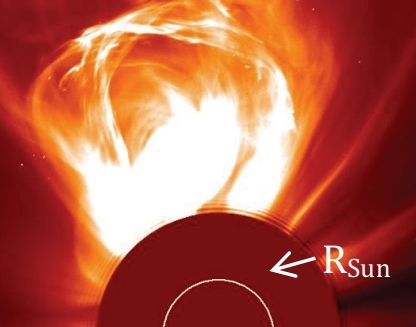
\includegraphics[width=0.4\textwidth]{hw4_p4.jpg} 
\end{center}

(a) What is the magnetic field strength of the flux rope required for local
pressure balance?

(b) The buoyancy of the flux rope causes it to rise. The flux rope breaks
through the Sun's surface and rises high into the corona. The surrounding
pressure drops to $10^{-5}$\,\si{Pa}. What is the magnetic field strength at
this point?

(c) What is the radius of the flux rope when it is high in the corona? Hint:
Magnetic flux, $BA$ where $A$ is area, is conserved. How does its size compare
to the radius of the Sun. $R_{\text{sun}}=7\times 10^5$\,\si{km}.

(d) The flux rope breaks out into the solar wind (see image). The surrounding
pressure is $10^{-7}$\,\si{Pa}. What is the magnetic field of the flux rope?

(e) What is the radius of the flux rope as it breaks out into the solar wind?

(f) Examine the CME image. Estimate the size of the CME based on the solar
radius. Does your calculation of the size of this flux rope match what is seen
in the CME image?
\begin{solution}
(a) The pressure internal and external to the flux rope is balanced. So we have
\begin{equation}
    P_{\text{ext}}=\frac{B^2}{2\mu_0}
    \Rightarrow
    B=\sqrt{2\mu_0P_\text{ext}}
    \approx0.5\,\si{T}
\end{equation}

(b) Using $P_{\text{ext}}=10^{-5}$\,\si{Pa}, the magnetic field at this point is
$B\approx 5$\,\si{\mu T}.

(c) The magnetic flux is conserved, so we can calculate the radius high in the
corona
\begin{equation}
    B_{\text{low}}\pi R_{\text{low}}^2=B_{\text{high}}\pi R_{\text{high}}^2
    \Rightarrow
    R_{\text{high}}=R_{\text{low}}\sqrt{\frac{B_{\text{low}}}{B_{\text{high}}}}
    \approx1.27\times 10^6\,\si{km}
    \approx 1.8R_{\text{sun}}
\end{equation}

(d) Similar to part (b), the magnetic field is $501$\,\si{nT}.

(e) From part (c), the radius as it breaks out into the solar wind is
\begin{equation}
    R_{sw}=R_{\text{low}} \sqrt{\frac{B_{\text{low}}}{B_{\text{sw}}}}
    \approx 5.7R_{\text{sun}}
\end{equation}

(f) This is on the same order of magnitude as the radius of the sun. So it is
comparable to the size seen in the image ($\approx 3-4 R_{\text{sun}}$).
\end{solution}
\end{problem}
%%%%%%%%%%%%%%%%%%%%%%%%%%%%%%%%%%%%%%%%%%%%%%%%%%%%%%%%%%%%%%%%%%%%%%%%%%%%%%%%
\end{document}
